\documentclass[12pt,a4paper,twopage,openright]{article}



% ******** vmargin settings *********
\usepackage{vmargin} %This give you full control over the used page area, it maybe not the idea method in Latex to do so, but I wanted to reduce to amount of white space on the page
\setpapersize{A4}
\setmargins{3.5cm}%			%linker Rand, left edge
	  {1cm}%     %oberer Rand, top edge
           {14.7cm}%		%Textbreite, text width
           {23.42cm}%   %Texthoehe, text hight
           {14pt}%			%Kopfzeilenhöhe, header hight
           {1cm}%   	  %Kopfzeilenabstand, header distance
           {0pt}%				%Fußzeilenhoehe footer hight
           {2cm}%    	  %Fusszeilenabstand, footer distance   


%Defining text font profile
\usepackage{t1enc} % as usual
\usepackage[latin1]{inputenc} % as usual
\usepackage{times}	
\usepackage{mathcomp}
\usepackage{amsmath}
\usepackage[pdftex]{graphicx}

\pagestyle{plain}
\renewcommand{\topfraction}{0.99}
\renewcommand{\bottomfraction}{0.99}
\renewcommand{\textfraction}{0}



\begin{document}
%Plan
%
\title{Analysis Methodology for Coaxial Wire Measurements of Impedance}
\author{Hugo Alistair Day}
\date{May 2010}
\maketitle


\begin{abstract}
The analysis of data from the measurement of device impedance using the coaxial wire technique require a degree of understanding of both what is actually being measured by the method, and of what is being defined as a real and imaginary impedance. Through my own work I discovered a lack of clear definitions of how the data measured directly related to the quantities that we refer to from the point of view of particle motion. The idea of this document is to attempt to clarify how the quantities are related, and also give a clear guide as to how to analyse the experimental data to be compatible with a beam dynamics point of view. This presently a work in progress
\end{abstract}

\newpage

\tableofcontents

% Introduction - Coaxial Wire Method
% Wakefield Basics - Definiton of longitudinal, dipolar/driving, quadrupolar/detuning impedance
% Analysis of transmission method
% Analysis of resonator method
%
The injection kicker magnets in the LHC are part of the injection system for the LHC machine. This system is used to match the trajectory of the injected beam to that of the stable beam path in the accelerator. An example schema for the LHC can be seen in Fig.~\ref{fig:injection-system-schema}. The system typically uses two components: a septum, which may provide a slowly rising and falling time, but strong, field, and kickers, which may provide a rapidly rising and falling, but comparatively weak, field to match the injected beam to the correct trajectory. Similar components are used for the fast extraction of beam (for systems such as the abort system) also.

\begin{figure}
\begin{center}
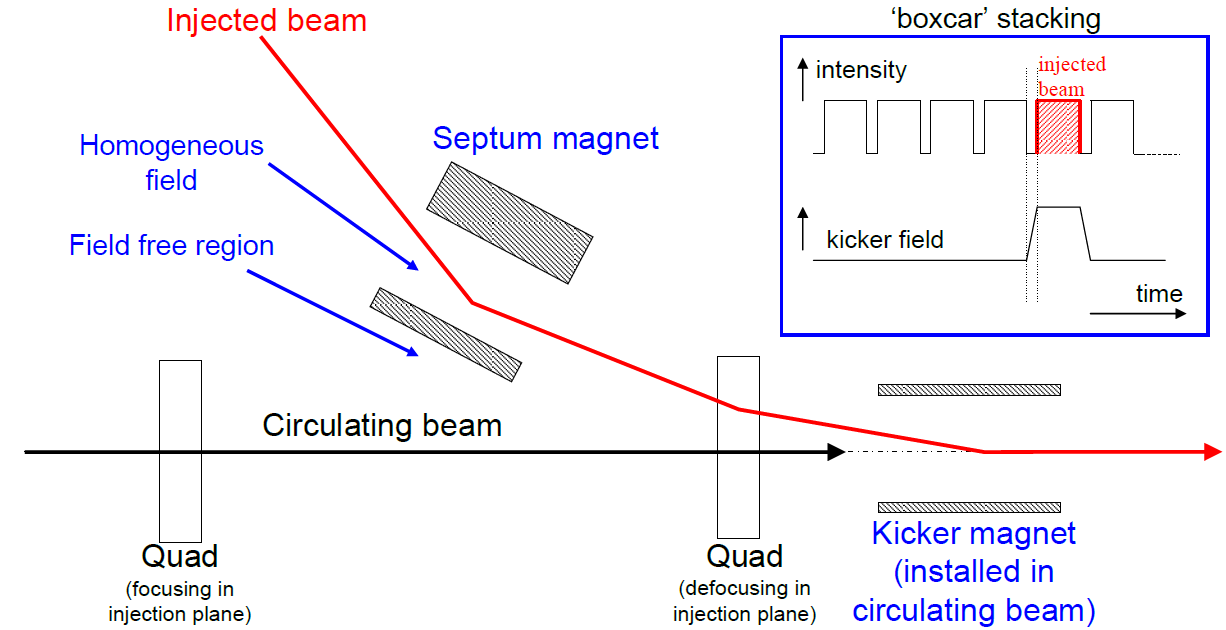
\includegraphics[width=0.6\textwidth]{LHC_MKI/figures/injection-system.png}
\end{center}
\caption{An example layout of a injection system for an accelerator. Taken from \cite{Barnes:injSys}}
\label{fig:injection-system-schema}
\end{figure}

By design kickers are generally always visible to the beam due to the need to quickly apply their kick. In order to achieve a fast field rise/fall time, the yoke of the kicker magnet is usually a NiZn ferrite. In addition the need for a highly homogeneous field whilst the kick is applied, as well as the strength of the field, neccesitates that the aperture for kickers often be relatively small, meaning they are in close proximity to the beam. This leads to two concerns - that the close proximity of the beam to such a device, that may be made of either a highly lossy material \cite{Day:wireMeasFerr, Barnes:wireMeasKick, Barnes:spsKickerHeating} or a source of strong geometrical impedance \cite{Belver-Aguilar:clicStripline}, may be source of impedance that drives instabilities in the beam \cite{Salvant:spsImpModel}, and secondly that the large real component of the ferrite ferrite may be subject to intense heating in high beam current machines \cite{Barnes:spsKickerHeating}. 

\section{LHC Injection Kicker Magnets}

Each LHC injection kicker magnet (LHC-MKI, or MKI) is a 3m long travelling wave transmission line kicker magnet (ferrite length 2.7m). For LHC there are two injection regions, near IPs 2 (ALICE) and 8 (LHCb), each consisting of a septa system and four MKIs injecting vertically into the machine (The position of the LHC injection systems is shown in Fig.~\ref{fig:lhc-injection-systems}). As a transmission line magnet the magnet is constructed of a c-core ferrite yoke, segmented by alternating HV and ground plates capacitively coupled together by ceramic capacitors to form a magnet of 5$\Omega$ characteristic impedance. The pulse is generated in a pulse forming network (PFN) and is subsequently carried by 10 parallel coaxial cables with a total characteristic impedance of $5 \Omega$, matching the characteristic impedance of the MKI and the PFN. The performance parameters of the magnets rise time, fied strength and homogeneity are given in Tab.~\ref{tab:mki-parameters} \cite{Ducimetiere:mkiSpec}.

\begin{figure}
\begin{center}
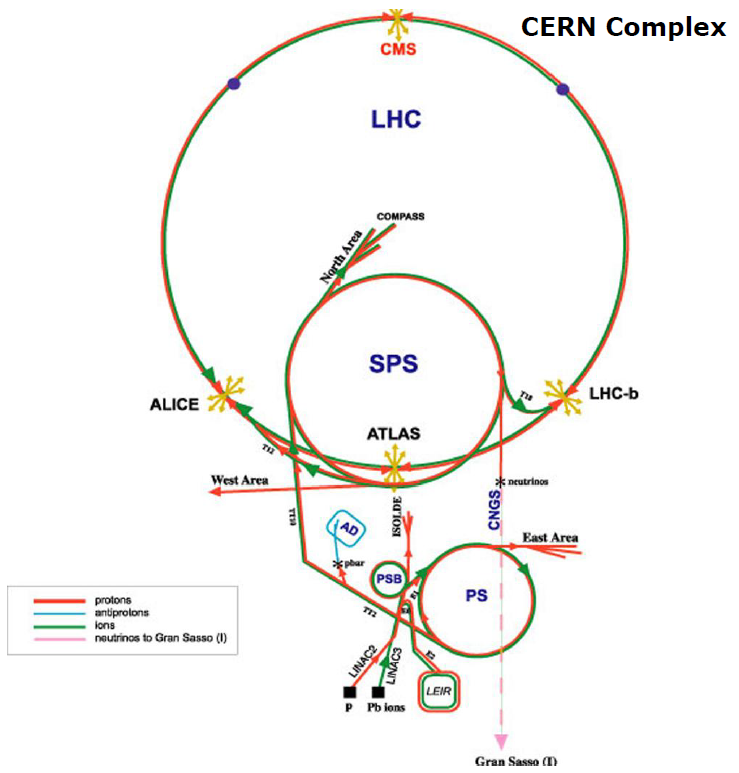
\includegraphics[width=0.75\textwidth]{LHC_MKI/figures/injection-points-lhc.png}
\end{center}
\caption{The location of the LHC injection systems in the LHC ring.}
\label{fig:lhc-injection-systems}
\end{figure}


\begin{figure}
\begin{center}
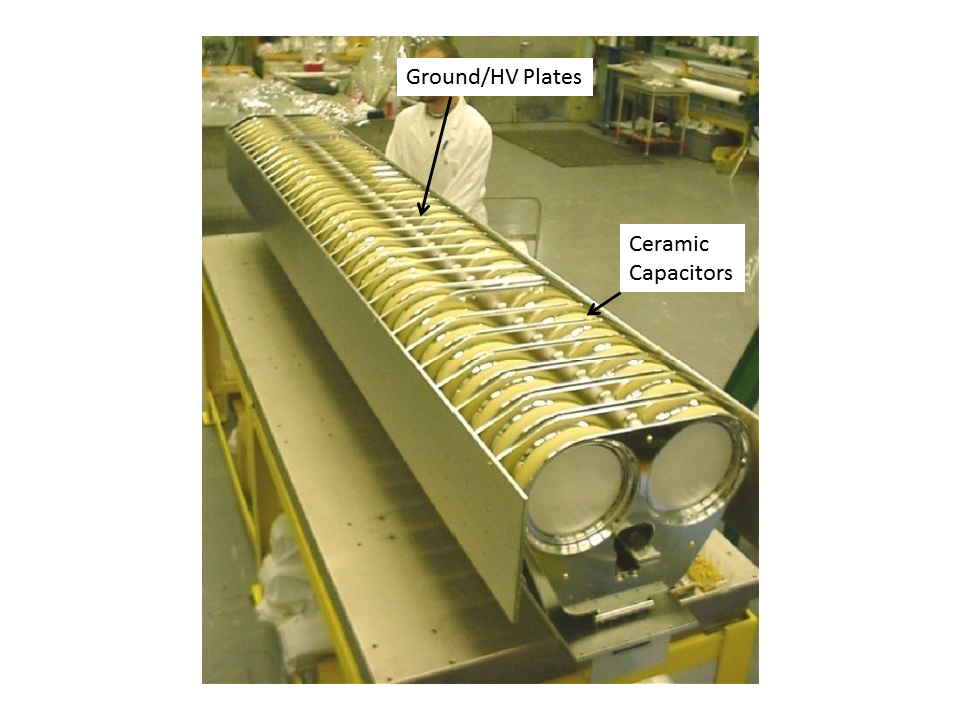
\includegraphics[height=0.4\textwidth]{LHC_MKI/figures/mki-out-vac-tank.png}
\end{center}
\caption{A cross section of an MKI. Visible are the alternating HV and ground plates, seperated by capacitor plates. The HV busbar and the ground return can be seen in the c core of the ferrite yoke.}
\label{fig:lhc-mki-cross-section}
\end{figure}

\begin{table}
\caption{MKI Operational parameters}

\begin{center}
\begin{tabular}{c | c | c}
Number of Kickers per System & 4 & \\ \hline
Kick strength per magnet & 0.3 & T.m \\ \hline
Beam aperture (diameter) & 38 & mm \\ \hline
Characteristic Impedance & 5 & $\Omega$ \\ \hline
Operating charging voltage (PFN) & 54 & kV \\ \hline
Field flat top ripple & < $\pm$0.5 & \% \\ \hline
Field flat top duration & up to 7.86 & $\mu$ s \\ \hline
Field rise time 0.5\%-99.5\% & 0.9 & $\mu$ s \\ \hline
Field fall time 99.5\%-0.5\% & 3.0 & $\mu$ s \\ \hline
Magnet kength & 2.7 & m \\ 
\end{tabular}
\end{center}
\label{tab:mki-parameters}
\end{table}
\section{Wakefield Basics}

Wakefields are a well researched phenomenon within accelerator physics, having first been discussed in the late 1950s, and continued research having developed the field to a mature level of understanding of the phenomenon. There is a wealth of literature describing the theoretical basis for the field [Chao/Zotter/Wilson/Masses] which will thus not be discussed in their entirity here. Here only the distinction between longitudinal, driving/dipolar and detuning/quadrupolar impedance will be made.

If we consider a lead particle of charge $q_{1}$ at a displacement $\vec{r_{1}} = (x_{1}, y_{1}, z = 0)$ following by a test particle of charge $q_{2}$ at a displacement $\vec{r_{2}} = (x_{2}, y_{2}, z = s)$ it is possible to solve Maxwell's equations for considering a generalised current density as is demonstrated in Chao [Chao - God of donkey]. This leads to the consideration of what are referred to as the wakefields, that is the electric fields that are induced behind (in the wake of) an inducing charged particle. These can be divided into both longitudinal fields and transverse fields, a distinction that will become significant later. We can represent these in terms of the electromagnetic fields in the structure as follows;

\begin{eqnarray}
W_{z}(r_{1},r_{2},s) & = & \frac{1}{q_{2}} \int_{z_{1}}^{z_{2}} [E_{z}(r_{2},z,t)]_{t=\frac{z+s}{c}}dz \\
\mathbf{W_{\perp}}(r_{1},r_{2},s) & = &\frac{1}{q_{2}} \int_{z_{1}}^{z^{2}} [\mathbf{E_{\perp}} + c(\hat{\mathbf{e_{x}}}  \times{}\mathbf{B}]_{t=\frac{z+s}{c}}dz
\label{eqn:wakefield-lorentz-trans}
\end{eqnarray}

where $W_{z}$ is the longitudinal wakefield, $W_{\perp}$ is the transverse wakefield, and $E_{z}$, $E_{\perp}$ and $B$ are the longitudinal electric field component, the transverse electric field components and the magnetic field respectively. 

Similarly, it is also convenient to consider the frequency domain properties of these fields, as many materials have a frequency dependant complex permitvitty and permeability. If we carry out a fourier transform on eqns 1 \& 2, we can derive a quantity known as the beam coupling impedance, or simply impedance for short;

\begin{equation}
Z(\omega) = \int^{\infty}_{-\infty} W(t) e^{-j\omega{}t} dt
\label{eqn:impedance-ft}
\end{equation}

It is subsequently possible to consider the impedance as a function of the m-th mode of a current density and the electric field of the system;

\begin{equation}
\bar{Z_{m}} = -\frac{1}{I^{2}} \int dV \mathbf{\bar{E_{m}}}\cdot\mathbf{\bar{J^{*}_{m}}}
\label{eqn:imp-modal}
\end{equation}

where

\begin{equation}
\bar{J_{m}} = \frac{I}{\pi{}a^{m+1}(1+\delta_{m0})} \delta{}(r-a)cos(m\theta)exp(j(\omega{}t-kz))\mathbf{e_{z}}
\label{eqn:j-def}
\end{equation}

This would subsequently produce an electromagnetic field $(\mathbf{\bar{E_{m}}}, \mathbf{\bar{H_{m}}})$. This definition has drawbacks however as it does allow for a current of the m-th mode to generate electric fields with different azimuthal components $sinn\theta$ and $cosn\theta$ ($n \not m$). To rectify this we can instead define the longitudinal coupling impedance as a convolution of modes given by

\begin{equation}
{Z_{m, n}} = -\frac{1}{I^{2}} \int dV \mathbf{E_{m}}\cdot\mathbf{J^{*}_{n}}
\label{eqn:imp-modal-coupled}
\end{equation}

where 

\begin{equation}
{J_{m}} = \frac{I}{2\pi{}a^{|m|+1}} \delta{}(r-a)exp(jm\theta)exp(j(\omega{}t-kz))\mathbf{e_{z}}
\label{eqn:j-def}
\end{equation}

You therefore have an electromagnetic field ($\mathbf{E_{m}}, \mathbf{H_{m}}$) generated by a current density $\mathbf{J_{m}}$ for a given mode m. Through some simple summation it is also possible to determine that

\begin{eqnarray}
\mathbf{\bar{J_{0}}} = \mathbf{J_{0}}, \\
\mathbf{\bar{J_{m}}} = \mathbf{J_{m} + J_{-m}}
\label{eqn:m-compare}
\end{eqnarray}

From this definition it can be determined that

\begin{eqnarray}
\bar{Z_{0}} &= Z_{0,0} \\
\bar{Z_{x}} &= \bar{Z_{1}} = Z_{1,1} + Z_{1,-1} + Z_{-1,1} + Z_{-1,-1} \\
\bar{Z_{y}} &= \bar{Z_{1}} \text{(with cos distribution replaced with sin)} = Z_{1,1} - Z_{1,-1} - Z_{-1,1} + Z_{-1,-1} \\
\bar{Z_{m}} &= Z_{m,m} + Z_{m,-m} + Z_{-m,m} + Z_{-m,-m}, m=1,2,...
\end{eqnarray}

From these definitions, if we consider the coupling impedance of a test particle at a transverse position ($x_{2} = a_{2}cos\theta_{2}$, $y_{2}=a_{2}sin\theta_{2}$) where the source current density is

\begin{equation}
J_{z} = I\delta(x-x_{1})\delta(y-y_{1})exp(j(\omega{}t-kz))
\end{equation}
\begin{equation}
= \sum^{\infty}_{m=-\infty}a_{1}^{|m|}exp(-jm\theta_{1})J_{m},
\end{equation}

at ($x_{1} = a_{1}cos\theta_{1}$, $y_{1}=a_{1}sin\theta_{1}$). The longitudinal impedance is then
\begin{flushright}
\begin{equation*}
Z = -\frac{1}{I^{2}} \int dV \left(\sum^{\infty}_{m =-\infty} a^{|m|}_{1} exp(-jm\theta_{1})E_{m}\right)\left(\sum^{\infty}_{n=-\infty} a_{2}^{n}exp(jn\theta_{2})J_{n}^{*}\right)
\end{equation*}

\begin{equation*}
=\sum_{m,n}a_{1}^{|m|}a_{2}^{|2|}exp(-jm\theta_{1})exp(jn\theta_{2})Z_{m,n}
\end{equation*}

\begin{equation*}
=Z_{0,0}+(x_{1}-jy_{1})Z_{1,0}+(x_{1}+jy_{1})Z_{-1,0}+(x_{2}+jy_{2})Z_{0,1}+(x_{2}-jy_{2})Z_{0,-1}
\end{equation*}

\begin{equation*}
+(x_{1}-jy_{1})^{2}Z_{2,0}+(x_{1}-jy_{1})(x_{2}-jy_{2})Z_{1,-1} + (x_2-jy_{2})^{2}Z_{0,-2}
\end{equation*}

\begin{equation*}
+(x_{1}-jy_{1})(x_{2}+jy_{2})Z_{1,1}+(x_{1}+jy_{1})(x_{2}-jy_{2})Z_{-1,-1}
\end{equation*}

\begin{equation*}
+(x_{1}+jy_{1})^{2}Z_{-2,0}+(x_{1}+jy_{1})(x_{2}+jy_{2})Z_{-1,1}+(x_{2}+jy_{2})^{2}Z_{0,2}
\end{equation*}

\begin{equation}
+O\left((x_{1},y_{1},x_{2},y_{2})^{3}\right)
\end{equation}
\end{flushright}

Similarly, the transverse impedance can be defined as 

\begin{equation}
\mathbf{Z_{\perp}} = \frac{j}{I^{2}}\int dV \left[\mathbf{E_{\perp}}+\mathbf{e_{z}} \times{} c\mu_{0}\mathbf{H_{\perp}}\right]
\end{equation}

Applying the Panofsky-Wenzel Theorem:

\begin{equation}
\mathbf{Z_{\perp}} = \frac{1}{k}\mathbf{\nabla_{\perp{}2}}Z
\label{eqn:panof-wen}
\end{equation}

we can obtain the transverse impedance;

\begin{flushleft}
\begin{align}
kZ_{x}&=\frac{\partial Z}{\partial x_{2}} = Z_{0,1}+Z_{0,-1}+(x_{1}-jy_{1})Z_{1,-1}+2(x_{2}-jy_{2})Z_{0,-2} + (x_{1}-jy_{1})Z_{1,1} +(x_{1}+jy_{1})Z_{-1,-1} \\ 
&+(x_{1}+jy_{1})Z_{-1,1} +2(x_{2}+jy_{2})Z_{0,2} +O((x_{1},y_{1},x_{2},y_{2})^{2})\\
&= Z_{0,1} +Z_{0,-1}+x_{1}\bar{Z_{x}}+jy_{1}(-Z_{1,-1} -Z_{1,1}+Z_{-1,-1}+Z_{-1,1}) +2x_{2}(
Z_{0,-2}+Z_{0,2})+j2y_{2}(-Z_{0,-2}+Z_{0,2}) + O((x_{1},y_{1},x_{2},y_{2})^{2})
\end{align}
\end{flushleft}

\begin{flushleft}
\begin{align}
kZ_{x}&=\frac{\partial Z}{\partial x_{2}} = jZ_{0,1}-jZ_{0,-1}-j(x_{1}-jy_{1})Z_{1,-1}-2j(x_{2}-jy_{2})Z_{0,-2} + j(x_{1}-jy_{1})Z_{1,1} -j(x_{1}+jy_{1})Z_{-1,-1} \\ 
&+j(x_{1}+jy_{1})Z_{-1,1} +2j(x_{2}+jy_{2})Z_{0,2} +O((x_{1},y_{1},x_{2},y_{2})^{2})\\
&= j(Z_{0,1} -Z_{0,-1})+y_{1}\bar{Z_{x}}+jx_{1}(-Z_{1,-1} +Z_{1,1}-Z_{-1,-1}+Z_{-1,1}) +2y_{2}(
Z_{0,-2}+Z_{0,2})+j2x_{2}(-Z_{0,-2}+Z_{0,2}) + O((x_{1},y_{1},x_{2},y_{2})^{2})
\end{align}
\end{flushleft}

The values of most importance are $\bar{Z_{x}}$ and $\bar{Z_{y}}$, so the transverse coupling impedance become $Z_{x} = x_{1}\bar{Z_{x}}/k, Z_{y} = y_{1}\bar{Z_{y}}/k$. 
\section{A Coaxial Wire as a Field Source}

To carry out the coaxial measurement, it is neccessary to use a thin conductive wire suspended in the device under test to simulate the electromagnetic fields as would be produced by a relativistic charged particle. Conveniently, the formalism as derived by Tsutsui is utilises a current density, which can represent either the motion of charged particle or of current carrying wire. This is subsequently utilised to simulate both two wire and single wire measurements.

\subsection{Two Wire Measurements}

If we consider two wires located at positions $x=\pm a$, their current density can be approximated by

\begin{align*}
J & = I(\delta(x-a)\-\delta(x+a))\delta(y)exp(j(\omega{}t - kz))\\
  & = \frac{I}{\pi{}a}\sum^{\infty}_{m=-\infty}exp(j(2m+1)\theta)exp(j(\omega{}t-kz))\\
  & = 2 \sum^{\infty}_{m=-\infty}a^{|2m+1|}J_{2m+1}
\end{align*}

The impedance is thus;

\begin{align}
Z & = -\frac{1}{I^{2}}\int dV \left( 2\sum^{\infty}_{m=-\infty}a^{|2m+1|}E_{2m+1}\right) \left( 2\sum^{n=\infty}_{n=-\infty}a^{|2n+1|}J^{*}_{2n+1}) \right)\\
& =  4\sum_{n,m} a^{|2m+1| + |2n+1|}Z_{2m+1,2n+1} \\
& =  4a^{2}(Z_{1,1} + Z_{-1,1} + Z_{1,-1} + Z_{-1,-1}) + O(a^{4})\\
& =  4a^{2}\bar{Z_{x}}+O(a^{4})
\end{align}

This demonstrates that the transverse impedance as defined in (2), $\bar{Z_{x}}/k$ can be measured using the two wire technique for negligable higher order components (i.e. small displacement a). Subsequently to determine the transverse impedance $\bar{Z^{\perp}_{x}}$ it is simply neccessary to utilise;

\begin{equation}
\bar{Z^{\perp}_{x}} = \frac{\bar{Z_{x}}}{k} = \frac{cZ}{\omega(2a)^{2}}
\end{equation}

where Z is the measured longitudinal impedance from the two wires.

\subsection{One Wire Measurements}

For a wire displaced at a distance $x=x_{0}$, $y=y_{0}$, the current density may be approximated as

\begin{align}
J & = & I\delta{}(x-x_{0})\delta{}(y-y_{0})exp(j(\omega t - kz)) \\
  & = & \frac{I}{2\pi a}\delta (r-a) \sum^{\infty}_{m=-\infty} exp(jm(\theta - \theta_{0})) exp(j(\omega t - kz)) \\
  & = & \sum^{\infty}_{m=-\infty} a^{|m|} exp(-jm\theta_{0})J_{m}
\end{align}

where

\begin{align*}
x_{0} = acos(\theta_{0}) \\
y_{0} = asin(\theta_{0})
\end{align*}

During measurements $a$ and $\theta_{0}$ will be varied and thus that various coefficients $Z_{n,m}$ can be determined.

\begin{align}
Z  &=  -\frac{1}{I^{2}}\int dV \left( \sum^{\infty}_{m=-\infty} a^{|m|} exp(-jm\theta_{0})E_{m} \right) \left( \sum^{\infty}_{n=-infty} a^{|n|} exp(jn\theta_{0}) J^{*}_{n} \right) \\
   &=  \sum_{m,n}a^{|m| + |n|}exp(-j(m-n)\theta_{0})Z_{m,n} \\
  &= Z_{0,0} + a \left[ exp(-j\theta_{0})(Z_{1,0} + Z_{0,-1}) + exp(j\theta_{0})(Z_{0,1}+Z_{-1,0} \right] \\
 & + a^{2} \ [ exp(-2j\theta_{0})(Z_{2,0} + Z_{1,-1} +Z_{0,-2}) + (Z_{1,1} + Z_{-1,-1}) \\
 & + exp(2j\theta_{0})(Z_{0,2} + Z_{-1,1} + Z_{-2,0}) ] \\
 & + a^{3} \left[...\right] + ...
\eqref{eqn:imp-gen}
\end{align}

By scanning the wire position, it is possible to obtain the values of the various coefficients and obtain the values for the transverse impedance. This will be covered in more depth in section 4.
\section{Analysis using the Transmission Method}

The transmission method of impedance measurement [ref Caspers/Kroyer/Mostacci] is the most frequently used method of taking data using the coaxial wire technique and has a number of technical difficulties associated with it that are well covered in the existing literiture [ref Caspers/Kroyer/Barnes/own notes]. Here we shall concern ourselves primarily with the analysis of the data collected which is less extensively covered. Firstly, we should clarify what the data measured actually is. These measurements involve the measurement of the scattering parameters of a signal passed through the device under test, in the case of this method the coefficient $S_{21}$ (as might be expected given the section title). This coefficient is a complex number, and on most visual network analysers (VNAs) can be outputted as a magnitude, an angle or a complex number. The subsequent analysis will assume that we are treating the complex number form, so note that if analysis is done seperately for the amplitude and the angle, \textbf{the same analysis method is valid for both values}. 

Firstly, to carry out the analysis we must convert the measured value, $S_{21}$, to a value which represents something to beam dynamics, the beam impedance. There are a number of methods in which this can be achieved through considering the scattering matrices for both lumped impedances or distributed impedances. This is covered in good detail in [Caspers/Kroyer SPS MKE paper].

For impedances that might be expected to be of a low value, or impedances located in a small physical space, the lumped impedance formula may be used; 

\begin{equation}
Z = 2Z_{ch} \frac{1-S_{21}}{S_{21}}
\end{equation}

For more distributed impedances there exist two log formulae which can be applied for differing conditions [ref Caspers/Jensen]

\begin{equation}
Z = -2Z_{ch}ln\left(\frac{S_{21,measured}}{S_{21,ref}} \right)
\label{eqn:log-form}
\end{equation}

where $S_{21,measured}$ is the measured transmission coefficient and $S_{21,ref}$ is the transmission coefficient of an equal length, perfectly conducting pipe. It should be noted that both $S_{21}$ values should be in linear format and not dB format for this analysis to be valid. The value of $Z_{ch}$ can be determined through either measurement of the reflection coefficient [Caspers] or by analytical results [RF ref]. \citation{eqn:log-form} can be simplified to

\begin{equation}
Z = -2Z_{ch}\left[ ln\left(Z\right) + i(\phi_{measured} - \phi_{ref}) \right]
\end{equation}

where $S_{21,measured} = Ze^{j\phi_{measured}}$ and $S_{21,ref}  = e^{j\phi_{ref}} = e^{j\frac{\omega L}{c}}$, $\phi_{measured}$ is the measured phase advance of the transmission coefficient, L is the length of the device being measured, c is the speed of light and $\omega$ is the angular frequency at which the measurement is carried out at.

[section on improved log formula and E. Jensen's paper]

An important note is that many VNAs will output phase measurements only between $-\pi < \phi_{measured} < \pi$ or $0 < \phi_{measured} < 2\pi$ whereas $\phi_{ref}$ may take values greater than this. It is neccessary to take account of this during data processing to prevent erroneous analyses.


\section{Analysis using the Resonator Method}

The resonator method of impedance measurement is an alternative measurement scheme for measuring the impedance of structures in which low power losses are to be expected. The method works by establishing a weak capacitive through coupling coupling between the VNA and the device under test (DUT) as shown in figure [figure: scheme of experiment]. This creates a standing wave oscillation within the DUT, from which Q values can be obtained from the $\lambda/2$ peaks that can be measured. Measurement of these Q values and a comparison to the expected Q values of a high conductive reference pipe allow the real impedance to be measured with very high accuracy. The imaginary impedance can also be meaured by the frequency shift of the Q values from that of a reference pipe by considering the increased electrical length of the DUT.

To develop a better understanding of how the resonator method works, let us consider the physical processes that occur within the DUT during measurements. Through the weak capacitive coupling, a series of standing waves is created within the DUT, with a wavelength;

\begin{equation}
\lambda = \frac{2 L_{electric}}{n}
\end{equation}

where $n$ is an integer and $L_{electric}$ is the electrical length of the DUT. At the corresponding frequencies to these wavelengths, it is possible to achieve very accurate measurements of the resistive losses of the transmitted signal due to their being minimal losses to surrounding frequencies. Using a lorentzian fitting routine to obtain the Q values of these peaks, the corresponding transmission coefficient is obtain and subsequently the real impedance. It is worth noting that if the DUT has a low enough impedance for the resonator method to be valid then the non-log formula (eqn [ref]) is valid even for distribbuted impedances.

To obtain the imaginary impedance, it is possible to utilise both the method described in section 4, or to measure the frequency shift of the resonant peaks between the DUT and a reference pipe. This reference pipe can either be calculated analytically or measured in a lab. If we consider the DUT in an electrical circuit, with the real impedance represented by a resistance $R_{1}$ and the imaginary impedance by an inductance $j\omega L$ and compare it to a circuit containing only a resistance $R_{2}$ we obtain two generic impedances;

\begin{align}
Z_{1} = R_{1} + j\omega L = R + jX = Z_{0,1}e^{j\phi} \\
Z_{2} = R_{2} = Z_{0,2}e^{j.0}
\end{align}

Subsequently if we consider the measured voltages of the two systems at any given time we measure;

\begin{align}
V_{1} = V_{0}e^{j(\omega_{1} t_{1} + \phi)} \\
V_{2} = V_{0}e^{j(\omega_{2} t_{2})}
\end{align}

As we are interested in the resonant peaks of the two measurements, i.e. were $V_{1} = V_{2} = V_{0}$, we can take the equivalence and determine $\phi$. Considering the real component of the voltage;

\begin{align}
V_{1} = V_{2} = V_{0} \\
V_{0}cos\left( \omega_{1}t_{1} + \phi\right) = V_{0}cos\left( \omega_{2}t_{2}\right) = V_{0}
\end{align}

Ergo,

\begin{align}
cos\left( \omega_{1}t_{1} + \phi\right) = cos\left( \omega_{2}t_{2}\right) \\
\omega_{1}t_{1} + \phi =  \omega_{2}t_{2} \\
\phi =  \omega_{1}t_{1} -  \omega_{2}t_{2}
\end{align}

The imaginary impedance can simply be measured through considering a complex impedance plane so that;

\begin{align}
X = Zsin(\phi) \\
X = \frac{Rsin{\phi}}{cos\phi} = Rtan\phi
\end{align} 
\section{Symmetric Structures}

The measurement of a symmetric structure greatly simplifies the measurement and analysis of the five impedance components considered significant for beam dynamics. A symmetric structure is defined as a structure that has both left/right and top/bottom symmetry in an orientation, as shown in figure [figure with ref]. It should be noted that this orientation does not have to be aligned with the reference orbit, however the respective impedances will have to be transformed to the correct coordinate system for any beam dynamics calculations if this is the case.

If we consider the single wire measurements, given a general description in formula \eqref{eqn:imp-gen}[eq 33], we can generalise the impedance to

\begin{equation}
Z = A_{1} + aexp(-j\theta) A_{2} + aexp(j\theta) A_{3} + a^{2}exp(-2j\theta) A_{4} + a^{2}exp(2j\theta) A_{5} + a^{2} A_{6}
% Generalised impedance proportional to x^2
\end{equation}

where $A_{1} = A_{0,0},$ $A_{2} = Z_{1,0} + Z_{0,-1}, $ $A_{3} = Z_{0,1} + Z_{-1,0}, $ $A_{4} = Z_{2,0} + Z_{1,-1} + Z_{0,-2}, $ $A_{5} = Z_{0,2} + Z_{-1,1} + Z_{-2,0}, $ $A_{6} = Z_{1,1} + Z_{-1,-1}$ and factors of $O(a^{3})$ are negligably small. It should be clear that $A_{1}$ is a representation of the longitudinal impedance, and the other combinations of the rotated measurements would be equal to the impedances $\bar{Z_{x}}$ and $\bar{Z_{y}}$ for certain values of $a$ and $\theta$. For example, if we set $a=x$ and $\theta  = 0$ in a cartesian coordinate system we obtain;

\begin{equation}
Z = A_{1} + x^{2}\left[A_{4} + A_{5} +A_{6}\right] = A_{1} + x^{2}\left[ \bar{Z_{x}} + \left(Z_{2,0} + Z_{0,2} + Z_{-2,0} + Z_{0,-2}\right) \right]
\end{equation}

where $\bar{Z_{x}} = Z_{1,1} + Z_{1,-1} + Z_{-1,1} + Z_{-1,-1}$. It can be seen that taking a series of measurements for different values of $x$ would give a parabola, of which the $x^{2}$ coefficient would be;

\begin{equation}
\bar{Z}_{l,1x} = \bar{Z_{x}} + \left(Z_{2,0} + Z_{0,2} + Z_{-2,0} + Z_{0,-2}\right)
\end{equation}

Using a similar derivation for $a=y$ and $\theta = \pi/2$ one can show that;

\begin{equation}
Z = A_{1} + y^{2}\left[\bar{Z_{y}} - \left(Z_{2,0} + Z_{0,2} + Z_{-2,0} + Z{0,-2}\right) \right]
\end{equation}

\begin{equation}
\bar{Z}_{l,1y} = \bar{Z_{y}} - \left(Z_{2,0} + Z_{0,2} + Z_{-2,0} + Z_{0,-2}\right)
\end{equation}

We define the detuning/quadrupolar impedance from this as

\begin{equation}
-kZ^{detuning} = \left(Z_{2,0} + Z_{0,2} + Z_{-2,0} + Z_{0,-2}\right)
\end{equation}

And as such the quadratic term coefficients can be rewritten as

\begin{align}
Z_{l,1x} = \bar{Z_{x}} - Z^{detuning} \\
Z_{l,1y} = \bar{Z_{y}} + Z^{detuning}
\end{align}

Given that we obtain $\bar{Z_{x}}, \bar{Z_{y}}$ directly from two wire measurements, we can thus obtain the detuning impedance by simply subtracting impedance from the two wire measurement from the quadratic coefficient $Z^{detuning} = \pm \left( Z_{l,1x/y} - \bar{Z_{y}} \right)$

Similarly, it can be seen that 

\begin{equation}
Z_{l,1x} + Z_{l,1y} = \bar{Z_{x}} + \bar{Z_{y}}
\end{equation}

which can act as a verification of the validity of the measurements taken.
\section{Asymmetric Structures}

Asymmetric structures are those that have only one plane of symmetry (top/bottom or left/right) or contain no planes of symmetry at all. These structures require a more complex approach to analysing the impedance to obtain the five desired components as it is neccessary to obtain the values for the 6 coefficients given in [eq 54]. To do this it is neccessary to carry out a scan of values of $a$ and $\theta$. By taking measurements of certain values it is possible to obtain the desired impedances. It should be noted that structures with only a slight assymmetry may still be measured using the procedure for symmtric structures, which may be preferable due to the changes to the experimental set up neccessary for measurements of asymmetric structures.

It is again possible to measure the driving impedances $Z_{x}^{driving},Z_{y}^{driving}$ by utlising the two wire measurement technique, which allows us to obtain $\bar{Z}_{x} = Z_{1,1} + Z_{1,-1} + Z_{-1,1} + Z_{-1,-1}$ and $ \bar{Z}_{y} = Z_{1,1} - Z_{1,-1} - Z_{-1,1} + Z_{-1,-1}$. Taking the same definition of $Z^{detuning}$ as

\begin{equation}
Z^{detuning} = \frac{-2\left(Z_{0,2} + Z_{0,-2}\right)}{k}
\end{equation}

where $k$ is the wavenumber of the transmission frequency. From the earlier definitions of $A_{4,5,6}$ it can thus be shown that

\begin{equation}
Z^{detuning} = \frac{Z_{x}^{driving} - Z_{y}^{driving}}{2} - \frac{A_{4} + A_{5}}{k}
\end{equation}

This indicates that it is only neccessary to obtain the values of $A_{4} + A_{5}$ as opposed to the values individually. By substituting a number of values into the generalised form of the longitudinal impedance it is possible to see that

\begin{equation}
A_{4} + A_{5} = \frac{Z(\theta = 0) + Z(\theta = \pi) - 2Z\left(\theta = \frac{\pi}{2}\right) - 2Z\left(\theta = \frac{3\pi}{2} \right)} {4a^{2}}
\end{equation}

for both the real and imaginary components of $A_{4} + A_{5}$. For corroboration of measurements it is advised to take readings a number of different values of $a$, but this is not neccessary if the results are determined accurate enough.

\bibliographystyle{IEEEtran}
\bibliography{general_bibliography}

\end{document}
